\documentclass[conference]{IEEEtran}
\usepackage{cite}
\usepackage{hyperref}
\usepackage{graphicx}
\usepackage{amsmath,amssymb,amsfonts,bm}
\usepackage{algorithmic}
\usepackage{textcomp}
\usepackage{xcolor}
\usepackage{subcaption}
\usepackage[justification=centering]{caption}

\newcommand*{\vertbar}{\rule[-1ex]{0.5pt}{1.5em}}
\newcommand*{\horzbar}{\rule[0.5ex]{1.5em}{0.5pt}}

\def\BibTeX{{\rm B\kern-.05em{\sc i\kern-.025em b}\kern-.08em
    T\kern-.1667em\lower.7ex\hbox{E}\kern-.125emX}}
\begin{document}

\title{Lossy Image Compression}

\author{Reed Foster}

\maketitle

\begin{abstract}
\end{abstract}

% \begin{IEEEkeywords}
% \end{IEEEkeywords}

\section{Introduction}

Image compression is an important area of study due to the ever-increasing consumption of media and explosion of big data image processing.
% Cite: Image Processing Principles and Applications (Tinku Acharya)
% Cite: something for increase in ML/CV on images
The goal of lossy image compression is to preserve the perceptually relevant portions of an image so that the image appears unaltered while drastically reducing the number of bits required to store the image.

In this paper, I will discuss several methods of image compression and evaluate their performance on metrics of image quality and compression ratio.

\section{Background}

\subsection{Perception}
Images are often represented as 3 separate channels of the red, green, and blue intensity at each pixel in the image.
However, because humans are more sensitive to some colors but not others, and are more sensitive to different hues when they are of different brightnesses or intensities, this is not the best way to encode images for compression.
JPEG uses the $YC_bC_r$ image representation, where $Y$ is the luma or brightness component and $C_b$ and $C_r$ are the blue and red difference components (i.e. $C_b = B - Y$, $C_r = R - Y$).
The human eye is most sensitive to the information in the $Y$ channel, but less sensitive to changes in red and blue color, so this leaves an opportunity to apply higher compression to the $C_b$ and $C_r$ channels to achieve higher compression ratios while maintaining similar image quality.

Humans perceive the different spatial frequencies in images with varying degrees of sensitivity.
% Cite: Human Visual System Based Wavelet Decomposition for Image Compression (Thomas O'Rourke)
State of the art lossy image compression systems (e.g. JPEG and JPEG2000 from the Joint Photographic Experts Group) leverage this to dramatically shrink the number of bits required to encode an image while maintaining a strong resemblance of the original image.
% Cite something from JPEG
In order to do this, the original image is transformed into a frequency representation and the frequency representation is quantized in order to reduce the number of bits required to store it.
The quantized frequency-domain representation is then passed through lossless entropy coding to produce a compressed bitstream that can be stored or transmitted and then decoded to reconstruct the original image.
The two most popular approaches for this transformation are the discrete cosine transform (DCT) and discrete wavelet transform (DWT).

\subsection{Discrete Transforms in 1D and 2D}

A frequency transform in general can be viewed as a series of inner products between the input function and a set of basis vectors.
Often, these basis vectors are chosen to be orthogonal (such as in the DCT and many variants of the DWT).
A one-dimensional transform of an input vector $\mathbf{x}$ can be represented as:

\begin{IEEEeqnarray}{rCl}
    \mathbf{\widetilde{x}} & = & \mathbf{\Phi}\mathbf{x} \\
    \mathbf{\Phi} & = & \begin{pmatrix}\horzbar~\bm{\varphi}^T_1~\horzbar\\\vdots\\\horzbar~\bm{\varphi}^T_N~\horzbar\end{pmatrix}
\end{IEEEeqnarray}

where $\bm{\varphi}_k$ are the basis vectors of the transform.
Each of the elements $\widetilde{x}_k$ of $\mathbf{\widetilde{x}}$ is a coefficient which measures the degree to which the input signal $\mathbf{x}$ is orthogonal to the corresponding basis vector $\bm{\varphi}_k$.
For a discrete fourier transform, these basis functions are simply complex exponentials, with different frequencies for different basis vectors:

\begin{equation}
    \bm{\varphi}_k = \begin{pmatrix} 1, e^{-\frac{2i\pi k}{N}}, e^{-\frac{4i\pi k}{N}}, \dots e^{\frac{2(N-1)\pi k}{N}} \end{pmatrix}^T
\end{equation}

Intuitively, a discrete transform of 2D data (e.g. a matrix) can be performed by first taking a discrete transform of each individual column:
\begin{equation}
    \mathbf{\widetilde{X}}_c = \begin{pmatrix}
        \horzbar~\bm{\varphi}^T_1~\horzbar\\\vdots\\\horzbar~\bm{\varphi}^T_N~\horzbar
    \end{pmatrix}
    \begin{pmatrix}
        \vertbar && \vertbar \\
        \mathbf{x}_1 & \dots & \mathbf{x}_N \\
        \vertbar && \vertbar \\
    \end{pmatrix}
\end{equation}

Then taking a discrete transform of each row of the partially transformed matrix:
\begin{IEEEeqnarray}{rCl}
    \mathbf{\widetilde{X}}^T & = & \mathbf{\Phi}\mathbf{\widetilde{X}}^T_c \\
    \mathbf{\widetilde{X}} & = & \mathbf{\Phi}\mathbf{X}\mathbf{\Phi}^T
\end{IEEEeqnarray}

\subsection{Discrete Cosine Transform and Discrete Wavelet Transform}

For a discrete cosine transform, the basis vectors are evenly spaced in frequency.
They are given by:

\[
    \bm{\varphi}_k = \begin{pmatrix} \cos\frac{\pi k}{2N}, \cos\frac{3\pi k}{2N}, \dots \cos\frac{(2N-1)\pi k}{2N} \end{pmatrix}^T
\]

The angular frequency of the $k$th basis vector is $k\pi/N$ and the phase offset is $k\pi/2N$.

\begin{figure}[htbp]
    %\centerline{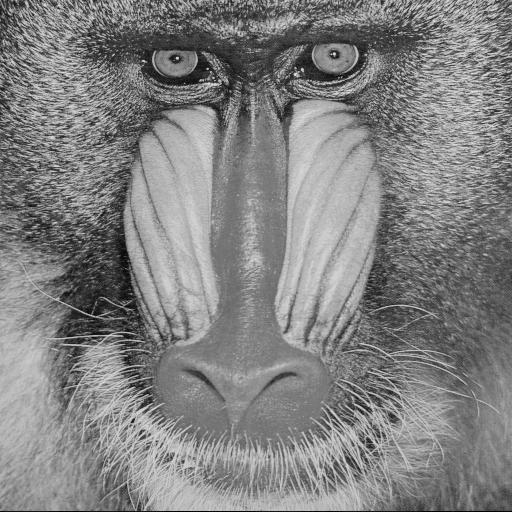
\includegraphics[width=0.8\columnwidth]{images/mandrill_gray.png}}
    \centering
    \begin{subfigure}{0.7\columnwidth}
        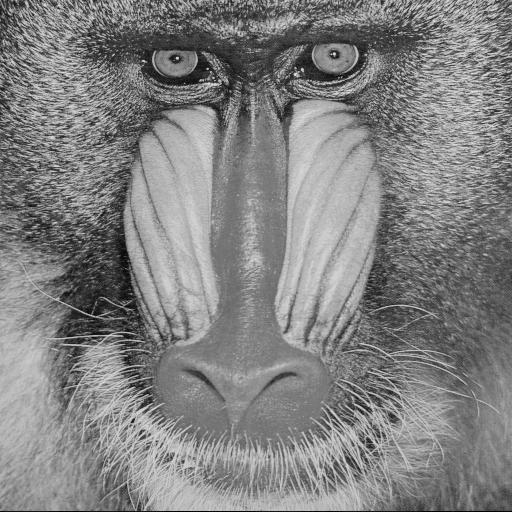
\includegraphics[width=\textwidth]{images/mandrill_gray.png}
        \caption{Grayscale Image of Mandrill}
        \label{fig:origGray}
    \end{subfigure}
    \par\bigskip
    \begin{subfigure}{0.7\columnwidth}
        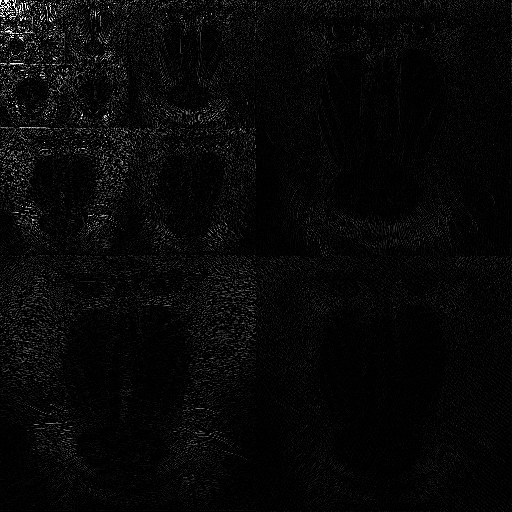
\includegraphics[width=\textwidth]{images/mandrill_linDWT.png}
        \caption{Linear Scale DWT of Image}
        \label{fig:linDWTGray}
    \end{subfigure}
    \par\bigskip
    \begin{subfigure}{0.7\columnwidth}
        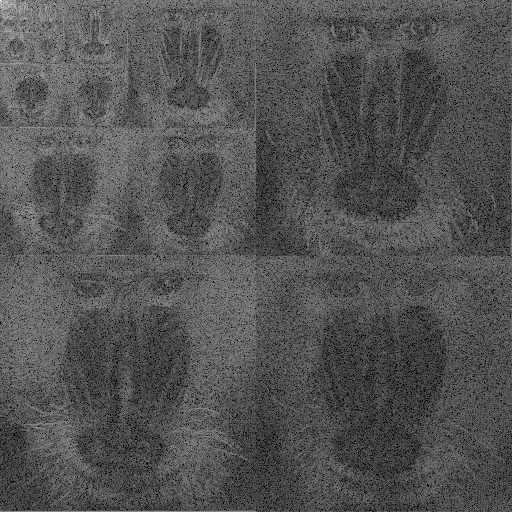
\includegraphics[width=\textwidth]{images/mandrill_logDWT.png}
        \caption{Log Scale DWT of Image}
        \label{fig:logDWTGray}
    \end{subfigure}
    \caption{Discrete Wavelet Transform of an image. The Cohen-Daubechies-Feauveau 9/7 (cdf97) wavelet used in JPEG2000 was selected for this transform.}
    \label{fig:dwtImage}
\end{figure}

Unlike the discrete cosine transform, which allocates equal bandwidth for each coefficient, discrete wavelet transform basis vectors (or wavelets) trade off frequency and spatial resolution.
The wavelets which have low frequency content (which will be maximally orthogonal to signals with low frequency and thus yield a large transform coefficient value) have poor spatial resolution but very fine frequency resolution.
Similarly, basis vectors with high frequency content are broadband in nature due to their temporally-localized structure.
% Cite: Julia Wavelets implementation?
The discrete wavelet transform is typically implemented as a set of cascaded filters and downsamplers.
The input signal is passed through a quadrature mirror filter consisting of a high pass and low pass filter.
Both filter outputs are decimated by a factor of 2, and the low pass filter output is recursively cascaded through another quadrature mirror filter pair.
This pattern of downsampling and recursively filtering the low pass output can be seen in Figure \ref{fig:logDWTGray}.
Because this is in two dimensions, each portion of the image is filtered twice: once by row and once by column.

\subsection{Singular Value Decomposition}

A matrix can be represented as a singular value decomposition.
Singular values $\sigma_i$ of a matrix $\mathbf{A}$ satisfy

\begin{equation}
    \mathbf{A}\mathbf{v}_i = \sigma_i\mathbf{u}_i
\end{equation}

with orthonormal $\mathbf{v}_i$ and $\mathbf{u}_i$ forming an eigenbasis for $\mathbf{A}^T\mathbf{A}$ and $\mathbf{AA}^T$ (respectively).
The singular value decomposition of an $m\times n$ matrix $\mathbf{A}$ of rank $r$ can be written as so

\begin{equation}
    \mathbf{A} = 
    \begin{pmatrix}
        \vertbar && \vertbar \\
        \mathbf{u}_1 & \cdots & \mathbf{u}_m \\
        \vertbar && \vertbar \\
    \end{pmatrix}
    \begin{pmatrix}
        \sigma_1 &&&\text{\Large0} \\ 
        & \ddots && \\
        && \sigma_r & \\
        \text{\Large0}&&& 0 \\
    \end{pmatrix}
    \begin{pmatrix}\horzbar~\bm{v}^T_1~\horzbar\\\vdots\\\horzbar~\bm{v}^T_n~\horzbar\end{pmatrix}
\end{equation}

Due to Eckart and Young, we know that the rank $k$ matrix $\mathbf{A}_k$ which is constructed from the first $k$ singular values of $\mathbf{A}$ minimizes the mean square error $\left\lVert\mathbf{A}-\mathbf{A}_k\right\rVert$.
% cite Eckart + Young

\begin{figure}[htbp]
    \centering
    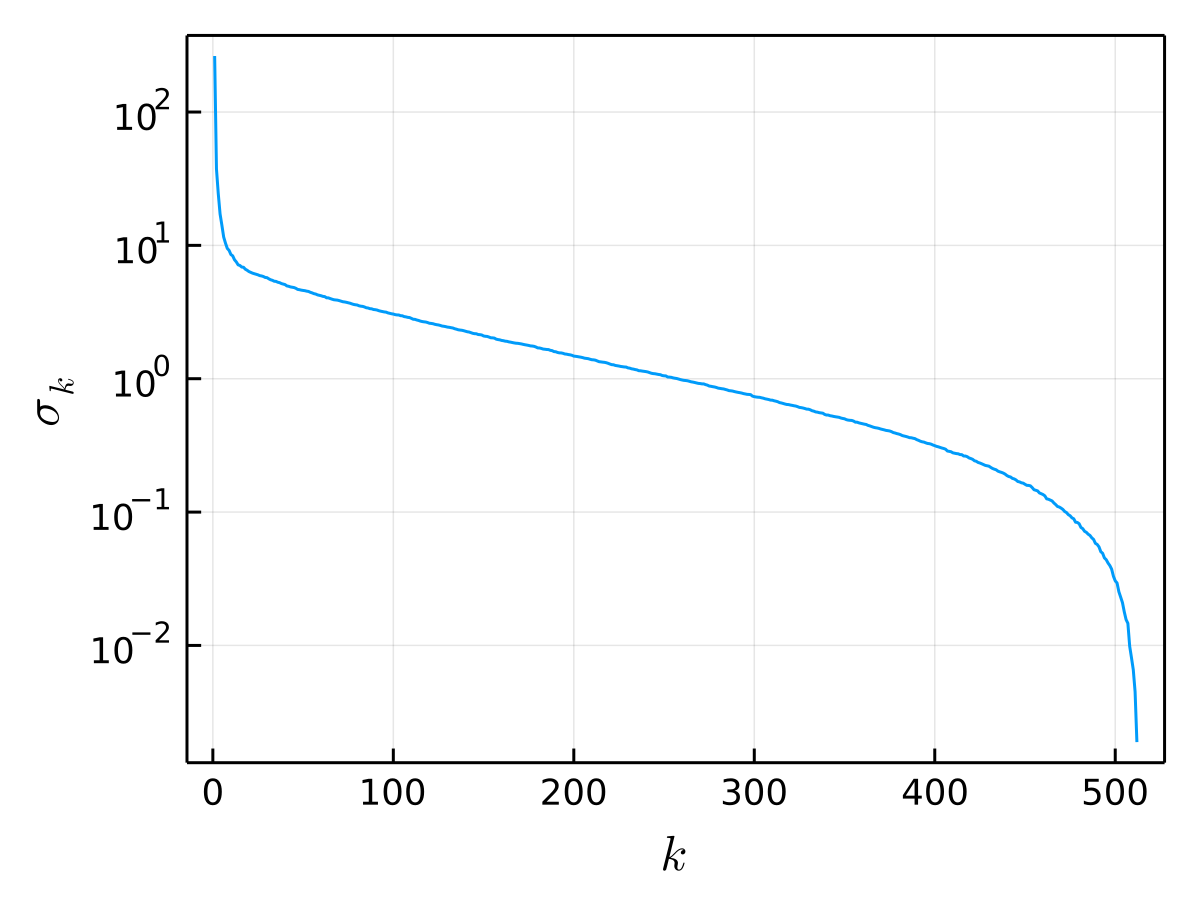
\includegraphics[width=0.7\columnwidth]{images/mandrill_SVD.png}
    \caption{Singular Values of Mandrill Image}
    \label{fig:svd}
\end{figure}


As shown in Figure \ref{fig:svd}, some singular values are very small compared to the largest singular values.
This leaves an opportunity for image compression through rank reduction.
The number of nonzero values required to store the SVD of a matrix can be calculated from the number of nonzero values in the 3 matrices of the SVD.
In $\mathbf{U}$, each basis vector $\mathbf{u}_i \in \mathbb{R}^m$ has $m$ elements.
For a rank $k$ truncation of the SVD, only $\mathbf{u}_1$ to $\mathbf{u}_k$ are needed, meaning $\mathbf{U}$ can be stored with $mk$ nonzero values.
Similarly, $nk$ nonzero values are required to store $\mathbf{V}^T$, and $k$ values to store the diagonal matrix of singular values $\bm{\Sigma}$.
Thus, the SVD can be compactly stored with $k(m + n + 1)$ nonzero values, provided $k \ll m,n$.
Storing the original $m\times n$ matrix of rank $r$ takes $mn$ nonzero values, so the rank-reduced SVD representation is not useful for compression if $k \approx m,n$.

\subsection{Lossless Compression - Entropy Coding}

The focus of this paper is not in entropy coding and lossless compression so there will be minimal discussion of these topics beyond this section.
Rank truncation and quantization reduce the number of nonzero values required to represent an image, but in order to actually store the information required to reconstruct the image, this sparsity must be leveraged by an entropy coding scheme.
JPEG (the 1992 standard) uses run length encoding and Huffman codes to create a compact representation of the quantized DCT representation of the image.
JPEG2000 uses arithmetic coding.
Because run length encoding is quite simple to understand and implement, I selected to also perform run length encoding and use the bitlength of a run-length-coded image as a compression ratio metric.
However, I will also report the sparsity of the transform-domain representation of the image (relative reduction in nonzero values in the image) as a compression ratio metric.

\section{Methods}

\subsection{Proposed Image Compression Techniques}

I implemented two DCT-based image compression techniques: one using the JPEG tiling and quantization scheme and one using an adaptive thresholding scheme.
I also implemented several DWT-based schemes.
I chose the Cohen-Daubechies-Feauveau 9/7 (cdf97) wavelet for computing the DWT because it is used in the JPEG2000 compression algorithm.
One is quite similar to JPEG2000, and uses scalar quantization.
Another uses the same adaptive thresholding scheme as in the DCT-thresholding compression technique.
I also implemented a rank-truncation method which uses the SVD of the transform-domain coefficients to compress the image.
Finally, I implemented a hybrid rank-truncation and adaptive thresholding method.

\subsection{Quantifying Image Quality}

The most common metric to quantify image quality is the mean squared error of the image, which is defined for a single channel as

\begin{equation}
    MSE_{1} = \frac{1}{mn}\sum_{m,n}\left(\mathbf{X}_{m,n} - \mathbf{\hat{X}}_{m,n}\right)^2
\end{equation}

where $\mathbf{X}$ is the original image and $\mathbf{\hat{X}}$ is the compressed image.
The mean squared error for the euclidean RGB distance between two colors is calculated as

\begin{equation}
    MSE_{RGB} = \frac{1}{3mn}\sum_{\mathbf{X}\in\{\mathbf{R},\mathbf{G},\mathbf{B}\}}\sum_{m,n}\left(\mathbf{X}_{m,n} - \mathbf{\hat{X}}_{m,n}\right)^2
\end{equation}

Finally, based on the perceptual model from CIE for $\Delta E$ (CIEDE2000), a metric of perceived color similarity, the perceived MSE can be calculated as

\begin{equation}
    MSE_{\Delta E} = \frac{1}{mn}\sum_{m,n}\Delta E\left(\mathbf{X}, \mathbf{\hat{X}}\right).^2
\end{equation}

where $\Delta E(\mathbf{X}, \mathbf{\hat{X}})$ computes the perceived difference between the 3-channel colors $\mathbf{X}$ and $\mathbf{\hat{X}}$.

Often, these mean squared error quantities are reported as a peak signal-to-noise ratio or PSNR:

\begin{equation}
    PSNR = 10\log_{10}\left(\frac{MAX_I^2}{MSE}\right)
\end{equation}

where $MAX_I$ is the maximum pixel value of the input $\mathbf{X}$ used to compute the mean squared error.

\subsection{Estimating Compression Ratio}

As mentioned in the section on Entropy Coding, the focus of this work is not on lossless compression techniques, so the compression ratio of these methods will be estimated with the relative increase in sparsity of the transform of the image and the number of bits required to store a run length encoding of the transform.

\section{Results}

\section{Discussion}

The IEEEtran class file is used to format your paper and style the text. All margins,
column widths, line spaces, and text fonts are prescribed; please do not
alter them. You may note peculiarities. For example, the head margin
measures proportionately more than is customary. This measurement
and others are deliberate, using specifications that anticipate your paper
as one part of the entire proceedings, and not as an independent document.
Please do not revise any of the current designations.

\section{Prepare Your Paper Before Styling}
Before you begin to format your paper, first write and save the content as a
separate text file. Complete all content and organizational editing before
formatting. Please note sections \ref{AA}--\ref{SCM} below for more information on
proofreading, spelling and grammar.

Keep your text and graphic files separate until after the text has been
formatted and styled. Do not number text heads---{\LaTeX} will do that
for you.

\subsection{Abbreviations and Acronyms}\label{AA}
Define abbreviations and acronyms the first time they are used in the text,
even after they have been defined in the abstract. Abbreviations such as
IEEE, SI, MKS, CGS, ac, dc, and rms do not have to be defined. Do not use
abbreviations in the title or heads unless they are unavoidable.

\subsection{Units}
\begin{itemize}
\item Use either SI (MKS) or CGS as primary units. (SI units are encouraged.) English units may be used as secondary units (in parentheses). An exception would be the use of English units as identifiers in trade, such as ``3.5-inch disk drive''.
\item Avoid combining SI and CGS units, such as current in amperes and magnetic field in oersteds. This often leads to confusion because equations do not balance dimensionally. If you must use mixed units, clearly state the units for each quantity that you use in an equation.
\item Do not mix complete spellings and abbreviations of units: ``Wb/m\textsuperscript{2}'' or ``webers per square meter'', not ``webers/m\textsuperscript{2}''. Spell out units when they appear in text: ``. . . a few henries'', not ``. . . a few H''.
\item Use a zero before decimal points: ``0.25'', not ``.25''. Use ``cm\textsuperscript{3}'', not ``cc''.)
\end{itemize}

\subsection{Equations}
Number equations consecutively. To make your
equations more compact, you may use the solidus (~/~), the exp function, or
appropriate exponents. Italicize Roman symbols for quantities and variables,
but not Greek symbols. Use a long dash rather than a hyphen for a minus
sign. Punctuate equations with commas or periods when they are part of a
sentence, as in:
\begin{equation}
a+b=\gamma\label{eq}
\end{equation}

Be sure that the
symbols in your equation have been defined before or immediately following
the equation. Use ``\eqref{eq}'', not ``Eq.~\eqref{eq}'' or ``equation \eqref{eq}'', except at
the beginning of a sentence: ``Equation \eqref{eq} is . . .''

\subsection{\LaTeX-Specific Advice}

Please use ``soft'' (e.g., \verb|\eqref{Eq}|) cross references instead
of ``hard'' references (e.g., \verb|(1)|). That will make it possible
to combine sections, add equations, or change the order of figures or
citations without having to go through the file line by line.

Please don't use the \verb|{eqnarray}| equation environment. Use
\verb|{align}| or \verb|{IEEEeqnarray}| instead. The \verb|{eqnarray}|
environment leaves unsightly spaces around relation symbols.

Please note that the \verb|{subequations}| environment in {\LaTeX}
will increment the main equation counter even when there are no
equation numbers displayed. If you forget that, you might write an
article in which the equation numbers skip from (17) to (20), causing
the copy editors to wonder if you've discovered a new method of
counting.

{\BibTeX} does not work by magic. It doesn't get the bibliographic
data from thin air but from .bib files. If you use {\BibTeX} to produce a
bibliography you must send the .bib files.

{\LaTeX} can't read your mind. If you assign the same label to a
subsubsection and a table, you might find that Table I has been cross
referenced as Table IV-B3.

{\LaTeX} does not have precognitive abilities. If you put a
\verb|\label| command before the command that updates the counter it's
supposed to be using, the label will pick up the last counter to be
cross referenced instead. In particular, a \verb|\label| command
should not go before the caption of a figure or a table.

Do not use \verb|\nonumber| inside the \verb|{array}| environment. It
will not stop equation numbers inside \verb|{array}| (there won't be
any anyway) and it might stop a wanted equation number in the
surrounding equation.

\subsection{Some Common Mistakes}\label{SCM}
\begin{itemize}
\item The word ``data'' is plural, not singular.
\item The subscript for the permeability of vacuum $\mu_{0}$, and other common scientific constants, is zero with subscript formatting, not a lowercase letter ``o''.
\item In American English, commas, semicolons, periods, question and exclamation marks are located within quotation marks only when a complete thought or name is cited, such as a title or full quotation. When quotation marks are used, instead of a bold or italic typeface, to highlight a word or phrase, punctuation should appear outside of the quotation marks. A parenthetical phrase or statement at the end of a sentence is punctuated outside of the closing parenthesis (like this). (A parenthetical sentence is punctuated within the parentheses.)
\item A graph within a graph is an ``inset'', not an ``insert''. The word alternatively is preferred to the word ``alternately'' (unless you really mean something that alternates).
\item Do not use the word ``essentially'' to mean ``approximately'' or ``effectively''.
\item In your paper title, if the words ``that uses'' can accurately replace the word ``using'', capitalize the ``u''; if not, keep using lower-cased.
\item Be aware of the different meanings of the homophones ``affect'' and ``effect'', ``complement'' and ``compliment'', ``discreet'' and ``discrete'', ``principal'' and ``principle''.
\item Do not confuse ``imply'' and ``infer''.
\item The prefix ``non'' is not a word; it should be joined to the word it modifies, usually without a hyphen.
\item There is no period after the ``et'' in the Latin abbreviation ``et al.''.
\item The abbreviation ``i.e.'' means ``that is'', and the abbreviation ``e.g.'' means ``for example''.
\end{itemize}
An excellent style manual for science writers is \cite{b7}.

\subsection{Authors and Affiliations}
\textbf{The class file is designed for, but not limited to, six authors.} A
minimum of one author is required for all conference articles. Author names
should be listed starting from left to right and then moving down to the
next line. This is the author sequence that will be used in future citations
and by indexing services. Names should not be listed in columns nor group by
affiliation. Please keep your affiliations as succinct as possible (for
example, do not differentiate among departments of the same organization).

\subsection{Identify the Headings}
Headings, or heads, are organizational devices that guide the reader through
your paper. There are two types: component heads and text heads.

Component heads identify the different components of your paper and are not
topically subordinate to each other. Examples include Acknowledgments and
References and, for these, the correct style to use is ``Heading 5''. Use
``figure caption'' for your Figure captions, and ``table head'' for your
table title. Run-in heads, such as ``Abstract'', will require you to apply a
style (in this case, italic) in addition to the style provided by the drop
down menu to differentiate the head from the text.

Text heads organize the topics on a relational, hierarchical basis. For
example, the paper title is the primary text head because all subsequent
material relates and elaborates on this one topic. If there are two or more
sub-topics, the next level head (uppercase Roman numerals) should be used
and, conversely, if there are not at least two sub-topics, then no subheads
should be introduced.

\subsection{Figures and Tables}
\paragraph{Positioning Figures and Tables} Place figures and tables at the top and
bottom of columns. Avoid placing them in the middle of columns. Large
figures and tables may span across both columns. Figure captions should be
below the figures; table heads should appear above the tables. Insert
figures and tables after they are cited in the text. Use the abbreviation
``Fig.~\ref{fig}'', even at the beginning of a sentence.

\begin{table}[htbp]
\caption{Table Type Styles}
\begin{center}
\begin{tabular}{|c|c|c|c|}
\hline
\textbf{Table}&\multicolumn{3}{|c|}{\textbf{Table Column Head}} \\
\cline{2-4}
\textbf{Head} & \textbf{\textit{Table column subhead}}& \textbf{\textit{Subhead}}& \textbf{\textit{Subhead}} \\
\hline
copy& More table copy$^{\mathrm{a}}$& &  \\
\hline
\multicolumn{4}{l}{$^{\mathrm{a}}$Sample of a Table footnote.}
\end{tabular}
\label{tab1}
\end{center}
\end{table}

\begin{figure}[htbp]
%\centerline{\includegraphics{fig1.png}}
\caption{Example of a figure caption.}
\label{fig}
\end{figure}

Figure Labels: Use 8 point Times New Roman for Figure labels. Use words
rather than symbols or abbreviations when writing Figure axis labels to
avoid confusing the reader. As an example, write the quantity
``Magnetization'', or ``Magnetization, M'', not just ``M''. If including
units in the label, present them within parentheses. Do not label axes only
with units. In the example, write ``Magnetization (A/m)'' or ``Magnetization
\{A[m(1)]\}'', not just ``A/m''. Do not label axes with a ratio of
quantities and units. For example, write ``Temperature (K)'', not
``Temperature/K''.

\section*{Acknowledgment}

The preferred spelling of the word ``acknowledgment'' in America is without
an ``e'' after the ``g''. Avoid the stilted expression ``one of us (R. B.
G.) thanks $\ldots$''. Instead, try ``R. B. G. thanks$\ldots$''. Put sponsor
acknowledgments in the unnumbered footnote on the first page.

\section*{References}

Please number citations consecutively within brackets \cite{b1}. The
sentence punctuation follows the bracket \cite{b2}. Refer simply to the reference
number, as in \cite{b3}---do not use ``Ref. \cite{b3}'' or ``reference \cite{b3}'' except at
the beginning of a sentence: ``Reference \cite{b3} was the first $\ldots$''

Number footnotes separately in superscripts. Place the actual footnote at
the bottom of the column in which it was cited. Do not put footnotes in the
abstract or reference list. Use letters for table footnotes.

Unless there are six authors or more give all authors' names; do not use
``et al.''. Papers that have not been published, even if they have been
submitted for publication, should be cited as ``unpublished'' \cite{b4}. Papers
that have been accepted for publication should be cited as ``in press'' \cite{b5}.
Capitalize only the first word in a paper title, except for proper nouns and
element symbols.

For papers published in translation journals, please give the English
citation first, followed by the original foreign-language citation \cite{b6}.

\begin{thebibliography}{00}
\bibitem{b1} G. Eason, B. Noble, and I. N. Sneddon, ``On certain integrals of Lipschitz-Hankel type involving products of Bessel functions,'' Phil. Trans. Roy. Soc. London, vol. A247, pp. 529--551, April 1955.
\bibitem{b2} J. Clerk Maxwell, A Treatise on Electricity and Magnetism, 3rd ed., vol. 2. Oxford: Clarendon, 1892, pp.68--73.
\bibitem{b3} I. S. Jacobs and C. P. Bean, ``Fine particles, thin films and exchange anisotropy,'' in Magnetism, vol. III, G. T. Rado and H. Suhl, Eds. New York: Academic, 1963, pp. 271--350.
\bibitem{b4} K. Elissa, ``Title of paper if known,'' unpublished.
\bibitem{b5} R. Nicole, ``Title of paper with only first word capitalized,'' J. Name Stand. Abbrev., in press.
\bibitem{b6} Y. Yorozu, M. Hirano, K. Oka, and Y. Tagawa, ``Electron spectroscopy studies on magneto-optical media and plastic substrate interface,'' IEEE Transl. J. Magn. Japan, vol. 2, pp. 740--741, August 1987 [Digests 9th Annual Conf. Magnetics Japan, p. 301, 1982].
\bibitem{b7} M. Young, The Technical Writer's Handbook. Mill Valley, CA: University Science, 1989.
\end{thebibliography}
\vspace{12pt}
\color{red}
IEEE conference templates contain guidance text for composing and formatting conference papers. Please ensure that all template text is removed from your conference paper prior to submission to the conference. Failure to remove the template text from your paper may result in your paper not being published.

\end{document}
